\ifx\twocol\undefined
\documentclass[12pt,letterpaper]{article}
\newcommand{\twocol}{0}
\else
\documentclass[8pt,twocolumn,letterpaper]{article}  % TWO COLUMN VERSION
\renewcommand{\twocol}{true}
\fi

\usepackage{amsmath}
\usepackage[pdftex]{color,graphicx}
\usepackage{verbatim}
\usepackage{setspace}
\usepackage{subfig}
\usepackage{algorithm}
\usepackage{algorithmicx}
\usepackage{algpseudocode}
\usepackage{ifthen}

% Include other packages here, before hyperref.

% If you comment hyperref and then uncomment it, you should delete
% egpaper.aux before re-running latex.  (Or just hit 'q' on the first latex
% run, let it finish, and you should be clear).
% \usepackage[pagebackref=true,breaklinks=true,letterpaper=true,colorlinks,bookmarks=false]{hyperref}
% \usepackage[colorlinks]{hyperref}

%%%THESIS%%% represent comment for thesis writing.
%\textcolor{red}{...}   represent comment for further elaborate.

% Define user command: This is for Bibliograph
\newcommand{\bbauth}[1]{\textrm{#1}}
\newcommand{\bbtitl}[1]{\textrm{#1}}
\newcommand{\bbjour}[1]{\textit{#1}}

%%%%%%%%%%%%%%%%%%%%%%%%%%%%%%%%
%%%%%%   GLOBAL SETTING  %%%%%%%
%%%%%%%%%%%%%%%%%%%%%%%%%%%%%%%%
\onehalfspace

\begin{document}
%%%%%%%%%%%%%%%%%%%%%%%%%%%%%%%%
%%%%%%   Title         %%%%%%%%%
%%%%%%%%%%%%%%%%%%%%%%%%%%%%%%%%
\title{\textbf{Lightweight 3D Reconstruction of Urban Buildings From Range Data}}
\author{
\\
by \\
\textbf{Weihong Li}
\\
\\
\\
Thesis Proposal for the degree of \\
\\
\textbf{Doctor of Philosophy} \\
\\
at the
\\
Graduate Center of the City University of New York \\
\\
\textbf{Advisor: George Wolberg}\\
\\
\\
\\
}
\date{April 2009}
\maketitle

\ifthenelse{\equal{\twocol}{true}}{
\tableofcontents
}{
\newpage % TWO COLUMN VERSION
\tableofcontents
\newpage % TWO COLUMN VERSION
}

%%%%%%%%%%%%%%%%%%%%%%%%%%%%%%%%
%%%%%%   ABSTRACT      %%%%%%%%%
%%%%%%%%%%%%%%%%%%%%%%%%%%%%%%%%
\section{Abstract}
Laser range scanners are widely used to acquire accurate scene measurements.
The massive point clouds they generate, however, present challenges to
efficient modeling, visualization, and storage.
State-of-the-art techniques for generating 3D models from voluminous
range data is well-known to demand large computational and storage requirements.
In this work, attention is directed to the modeling of urban buildings
directly from range data.
We propose an efficient modeling algorithm that exploits \emph{a priori}
knowledge that buildings can be modeled using extrusion and taper operations
to cross-sectional contours.
Inspired by this simplicity, we identify key cross-sectional slices among
the point cloud that consist of salient features.
Standard image processing algorithms are used to remove noise, fill holes,
and vectorize the projected points into contours.
Applying extrusion and taper operations to these contours
permits us to achieve dramatic geometry compression, making the resulting
models suitable for web-based applications such as Google Earth
or Microsoft Virtual Earth.
This work has applications in architecture, urban design, virtual city
touring, and online gaming.
The preliminary results on exterior urban building dataset are presented to
validate the proposed approach.


%%%%%%%%%%%%%%%%%%%%%%%%%%%%%%%%
%%%%%%   INTRODUCTION  %%%%%%%%%
%%%%%%%%%%%%%%%%%%%%%%%%%%%%%%%%
\ifthenelse{\equal{\twocol}{true}}{
%\newpage % TWO COLUMN VERSION
}{
\newpage % TWO COLUMN VERSION
}
\section{Background, Motivation and Research Goals}
Automatic 3D modeling of urban buildings is an area of active research
with increasing attention drawn from the computer graphics and
computer vision communities.
Current state-of-the-art algorithms for 3D modeling of urban buildings are
computationally expensive and suffer under the weight of large-scale datasets.
Despite a recent thrust of activity in 3D modeling and visualization of
urban buildings for web-based applications such as Google Earth and Microsoft
Virtual Earth, much 3D modeling continues to be manually generated.
Applications such as Google SketchUp are popular tools for creating
3D models of urban buildings via an intuitive push-pull modeling interface.
This process, however, remains tedious, expensive, and generally produces
low-resolution results.
This work seeks to introduce an automatic and efficient algorithm for
generating lightweight 3D models of urban buildings directly from point clouds.

The proposed algorithm can generate models across a wide spectrum of
resolutions.
A particularly useful feature of the algorithm is that even for a low
resolution model, the sharpness of the raw data is preserved, thereby
outperforming most of the existing approximation techniques.
The contribution of this work is that it combines the benefits of
\emph{a priori} knowledge of urban buildings and lightweight 2D image
processing techniques to perform 3D modeling of urban buildings directly
from point cloud data.
This offers the benefit of a cost-effective geometry compression
approach for voluminous range data.
It can be applied to boost web-based 3D applications, including
Google Earth, Microsoft Virtual Earth, virtual city touring and online gaming.

%%%%%%%%%%%%%%%%%%%%%%%%%%%%%%%%
%%%%%% Related Work    %%%%%%%%%
%%%%%%%%%%%%%%%%%%%%%%%%%%%%%%%%
%\section{Related Work}

% Refer to the following questions for writting.
% In \cite{RE_TOGSH}, what's been done, what approaches are proposed, what's the prons and cons.

In an attempt to steer clear of tedious and expensive hand-made models,
procedural modeling of buildings in \cite{PMB_MWH,PMB_WWS,PMB_PM} has been proposed.
By using an effective description language, buildings and streets of a virtual
city can be generated automatically.
The strength of this approach is that the description language can generate
a huge number of buildings and streets quickly and beautifully.
This is particular useful for gaming or other computer graphics applications.
However, since the parameters used to generate the buildings are randomly
generated, the city generated with these buildings and streets is a virtual one.
This approach is not useful for attempting to model an {\it existing} building.
In order to do so, one has to manually specify the parameters of the building,
which is very cumbersome.
Our goal is to automatically infer the parameters of an existing building and
therefore reproduce it quickly using the procedural modeling language
described above.

%%% Figure of the tapered template.
\ifthenelse{\equal{\twocol}{true}}{
\begin{figure} [h] % TWO COLUMN VERSION
}{
\begin{figure} [hbtp]
}
  \subfloat[]{
    \label{fig_IR_2_DXF:a} %% label for first subfigure
    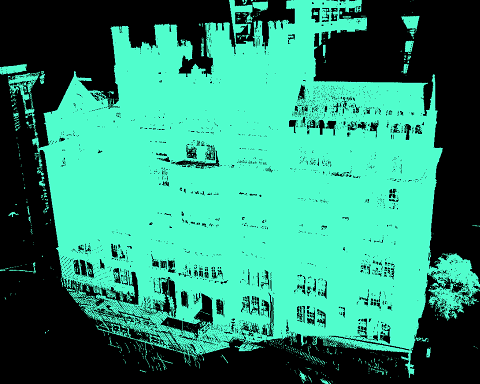
\includegraphics
        [width=0.5\textwidth]
	{figures/point_cloud.png}
  }
  \centering
  \subfloat[]{
    \label{fig_IR_2_DXF:b} %% label for first subfigure
    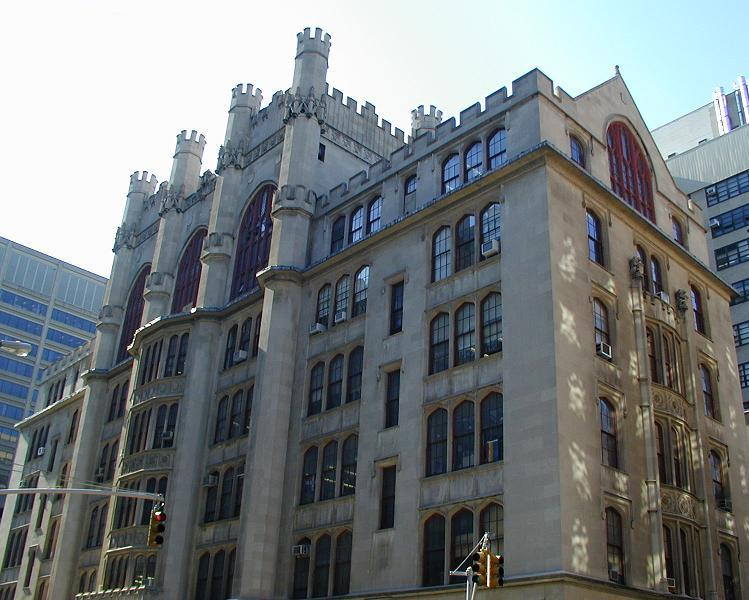
\includegraphics
        [width=0.5\textwidth]
	{figures/HunterPhoto.jpg}
  }
  \vspace{.1in}
  \subfloat[]{
    \label{fig_IR_2_DXF:c} %% label for first subfigure
    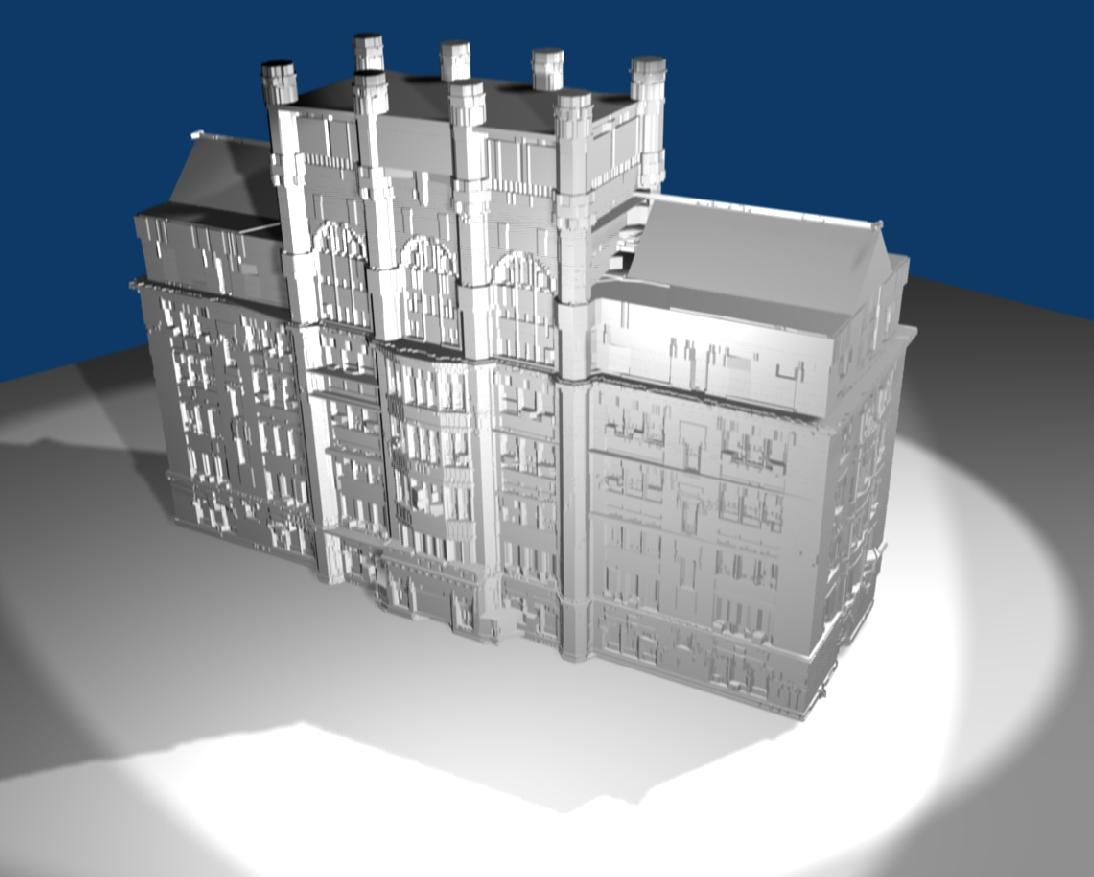
\includegraphics
        [width=0.5\textwidth]
	{figures/HunterShaded.jpg}
  }
  \centering
  \subfloat[]{
    \label{fig_IR_2_DXF:d} %% label for first subfigure
    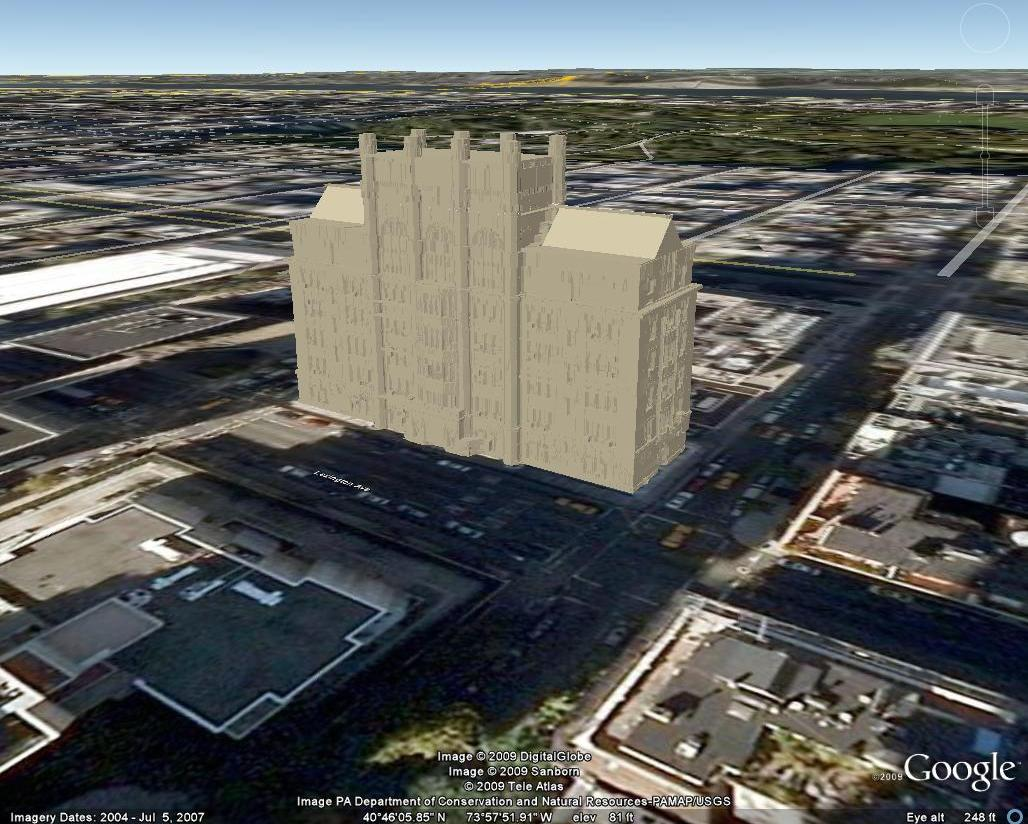
\includegraphics
        [width=0.5\textwidth]
	{figures/HunterGE.jpg}
  }
  \caption{ 3D point cloud and its reconstructed model of a building.
(a) A snapshot of the registered multiple scanning 3D point cloud data.
(b) The photo of the building.
(c) The reconstructed 3D model.
(d) The placement of the 3D model on Google Earth.
}
  \label{fig_IR_2_DXF}
\end{figure}
%%% End of Figure


There has been a lot of related work on 3D reconstruction in the research
community.
Essentially, this reconstruction process is the reverse engineering problem
of computer graphics \cite{RE_Fisher,RE_CLF,RE_CD}.
Reverse engineering of range data has been applied in numerous research areas,
including computer-aided design (CAD), computer vision, architectural modeling,
and medical image processing.
In \cite{DP_OWYC}, Or et al. proposed a 3D building reconstruction from a 2D floorplan image.
With the help of 2D
floorplan image, both the interior and exterior of a building are reconstructed accordingly.
However, the unavailability of 2D floor plan makes this approach not applicable to most applications,
including our project.
In \cite{RE_TOGSH}, Thompson et al. made use of known manufacturing features
to infer the 3D structure of the mechanical parts.
Their method benefits from the domain knowledge that most of the mechanical
parts consist of predefined structures, such as holes, bosses, and grooves.
Our work is partially motivated by this idea since it also incorporates
{\it a priori} knowledge about the construction of urban buildings for further
inference.
However, their method is based on predefined simple geometry structures and
the assumption that the input 3D data has a high signal-to-noise (SNR) ratio.
This hinders their approach for those applications with low SNR and
incomplete data.

Medical image processing techniques, on the other hand, usually deal with
low SNR data.
There has been a lot of work on medical 3D image reconstruction as in
\cite{MIR_FJS,MIR_BMMNB,MIR_KL,MIR_SKJ,MIR_SMHC,MIR_BVC}.
The basic idea behind the vast amount of work conducted in this area is 3D
reconstruction from sliced or histologic images using interpolation techniques.
Statistical inference is also extensively used to infer the low SNR images.
For example, in \cite{MIR_FJS}, Sigworth addressed the problem of low SNR
images using the maximum-likehood approach.
Most of these statistical processes are computationally intensive
in order to obtain accurate, high resolution models.

We propose an efficient way to reconstruct 3D models from range data by
partitioning the data into thin cross-sectional slabs of volume.
For each slab, all range data in that slab is projected onto a 2D
cross-sectional image slice.
Producing this array of slices permits us to avoid direct computation on
3D data, which is time-consuming and computationally complex.
A similarity measure \cite{IR_Brown,IR_ZF,RE_WWLZ} can be used to cluster the sliced images
together into {\it keyslices}.
This term is analogous to ''keyframes'' in computer animation, which denote
important moments in the animation sequence from which intermediate results
can be derived.
Each keyslice is a 2D image which contains the salient cross-sectional
structure of a building.
We leverage fast 2D image processing techniques on these keyslices
to produce lightweight 3D models, consisting of only a few hundred polygons.

To generate the 3D model of a building, all these keyslices need to be vectorized to
represent the silhouette or boundary of the building. Couple of raster image vectorization approaches are
proposed in \cite{DP_AAKMT,DP_DP,DP_WM}. The Douglas-Peucker
algorithm tried to connect all the existed points to form a polygon. Although the implementation of
this approach is very efficient with the improvement in \cite{DP_HS},  this method cannot
handle the case where some extra interior points are existed as some outlier data.
To tackle this issue, we proposed an adaptive ball-pivot algorithm (BPA) which was
original proposed on 3D point cloud data, on the 2D image to obtain
vectorized contours.


%%%%%%%%%%%%%%%%%%%%%%%%%%%%%%%%
%%%%%%   METHODS  %%%%%%%%%%%%%%
%%%%%%%%%%%%%%%%%%%%%%%%%%%%%%%%
\ifthenelse{\equal{\twocol}{true}}{
%\newpage % TWO COLUMN VERSION
}{
\newpage % TWO COLUMN VERSION
}
\section{Research Plan and Methodologies}

The approach we proposed for 3D modeling of urban building consists of
3 stages as shown in Figure \ref{fig_flow}.
First of all, the coordinates of the 3D point cloud stored in ascii format are loaded into memory.
To carry out lightweight process, the 3D point data
is projected to a serial of 2D image slices to avoid computation on 3D data directly.
Due to the occlusion and some special structures of the building, such as windows, the input data
is not complete and contains outlier noise.
Therefore, the noise removal and missing data recovering are carried out as a pre-processing stage to
generate the 3D model.  These will be addressed in the Section \ref{sec_mdr}.

\begin{figure}[htb]
  \centering
  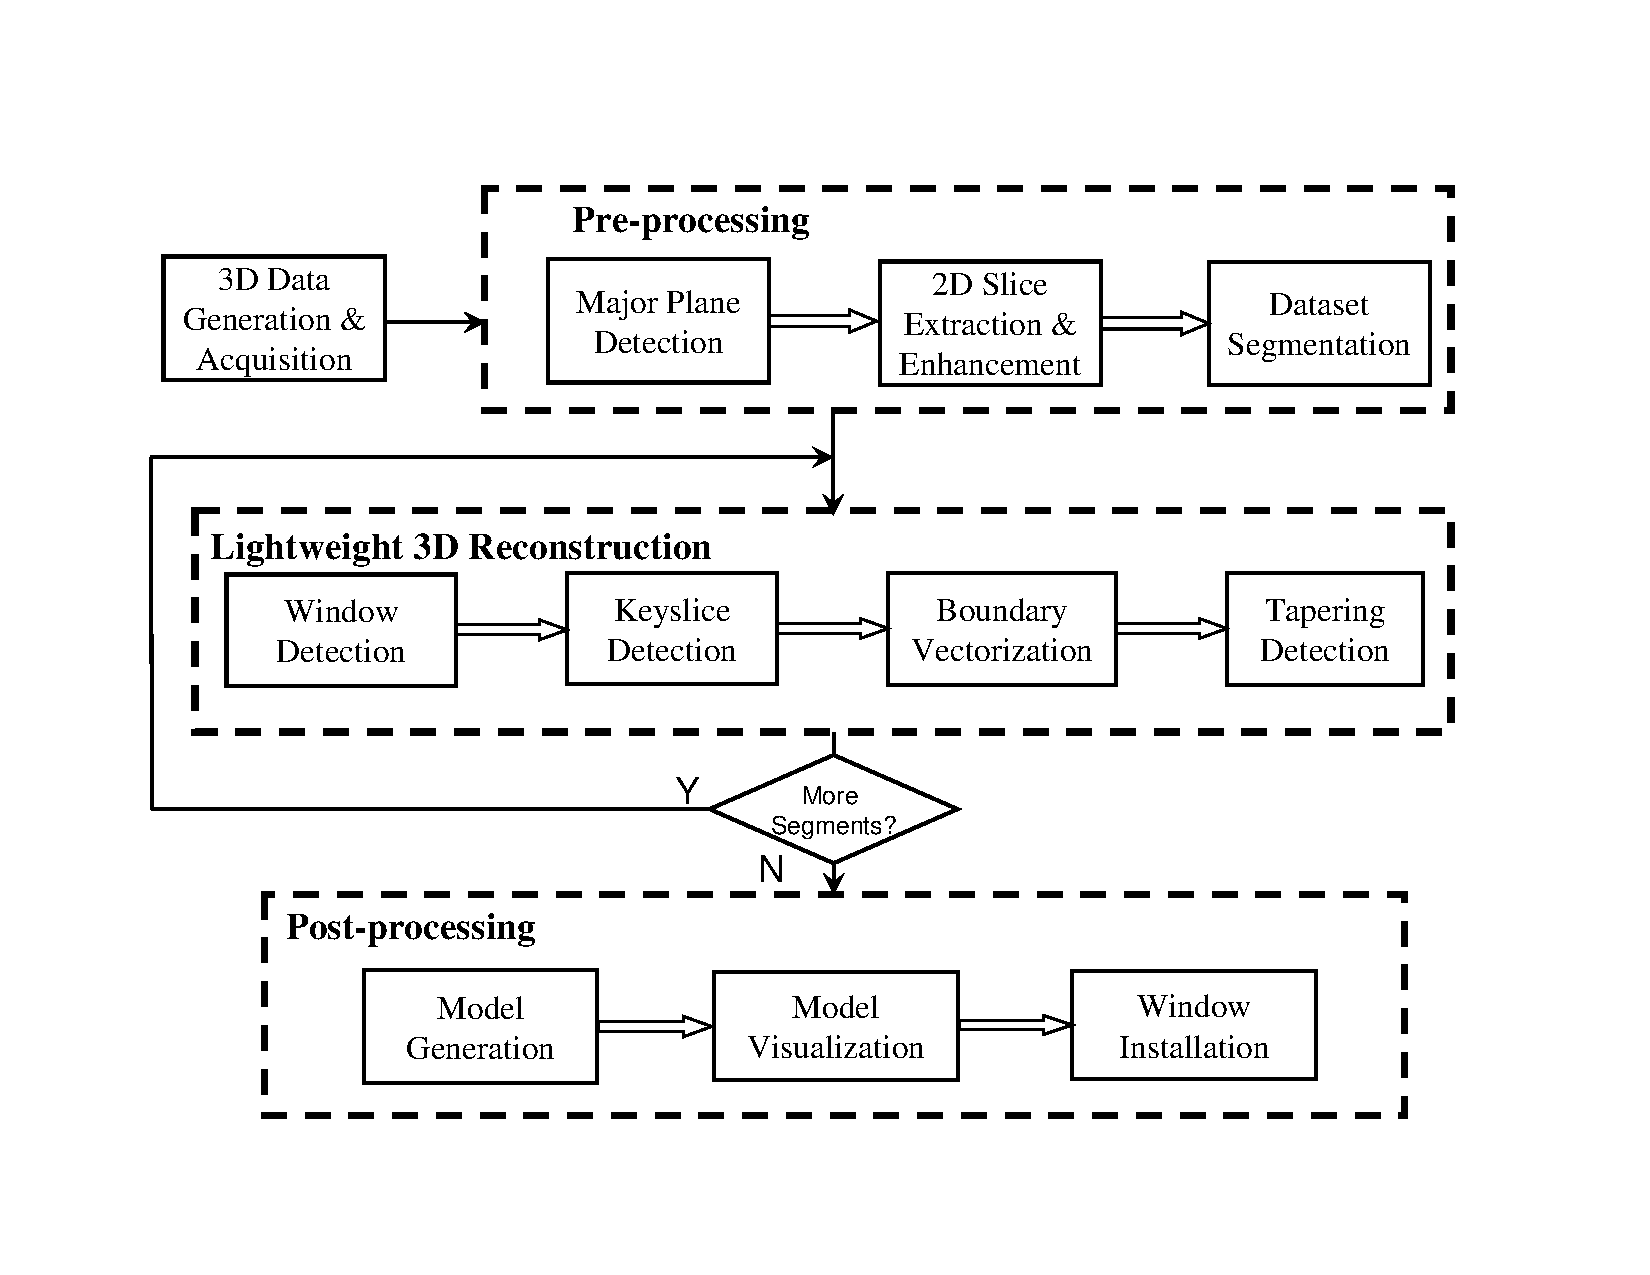
\includegraphics
      [width=\textwidth]
      {figures/flow.pdf}
      \caption{Flow graph for proposed approach}
      \label{fig_flow}
\end{figure}

The next stage of the approach is to carry out lightweight
image processing techniques on the enhanced image slices.
As mentioned before, the goal is to reconstruct the 3D
model from the point cloud based on the extruded and tapered
operation. Extrusion detection will cluster the above 2D slices into keyslices, which will
be used for further modeling processing.
After this, boundary vectorization for these raster
keyslices will be conducted. Section \ref{sec_ksd} and
Section \ref{sec_BPA} will describe the algorithms and implementations on the keyslices
detection and boundary vectorization. Tapered structure detection is carried out to
further reduce the model size.

For the final 3D model generation and visualization purpose, the inferred 2D information will
be transformed back to 3D world coordinate system, which is the last stage of the proposed approach.
Once all the above steps are completed, a 3D models of urban buildings is reconstructed
from its range data. Figure \ref{fig_IR_2_DXF}\subref{fig_IR_2_DXF:c}
shows an example of a 3D reconstructed model. This model can be easily placed on web-based
application, such as Google Earth as depicted in Figure \ref{fig_IR_2_DXF}\subref{fig_IR_2_DXF:d}.

%%%%%%%%%%%%%%%%%%%%%%%%%%%%%%%%
%%%%%%   PREPRCESSING  %%%%%%%%%
%%%%%%%%%%%%%%%%%%%%%%%%%%%%%%%%
\subsection{3D Point Cloud Preprocessing}
\label{sec_prep}
The input to our system is range data assembled as a 3D point cloud.
Our data is obtained from a Leica Cyrax 2500 laser range scanner \cite{RDP_LRS},
which works by sweeping an eye-safe laser beam across the scene to collect
up to one million 3D depth points per frame.
All scene points that lie within 100 meters can be acquired with an accuracy
of 5mm in depth.
The basic algorithm that we use for registering the voluminous 3D data
acquired from multiple scans of buildings has been introduced in
\cite{RDP_LS}.
Figure \ref{fig_IR_2_DXF}\subref{fig_IR_2_DXF:a} shows a snapshot of the
registered 3D point cloud, consisting of 14 scans totalling 14 million points.

Due to occlusions and limited vantage points, the point cloud collected by the
laser scanner \cite{RDP_LRS} contains noise and missing data.
In addition, computing directly on 3D data is time-consuming and
computationally complex.
To tackle these issues, we define inner and outer bounding boxes for the
building to clip away unrelated scene objects.
Then, we convert the 3D modeling problem into a set of 2D problems by
projecting the 3D data into a series of 2D cross-sectional images.
Noise removal, hole filling, and vectorization are all done in this
2D space.

\subsection{Extraction of 2D Slices}
\label{sec_image_slicing}
We consider the point cloud data as a large array of 3D points that can be
sliced into horizontal slabs of volume.
All 3D points within each slab will be projected onto a horizontal cutting
plane, or slice, at the base of the slab.
The height of each slab is $\boldsymbol{\delta}$.
If that value is held constant, each slice is generated from equal-sized
slab intervals.
If $\boldsymbol{\delta}$ is allowed to be a dynamic value, then we may
choose to allow for large values in parts of the structure that are similar,
and low values in regions that contain finer detail.
To avoid working on 3D data directly, a relatively small constant value
for $\boldsymbol{\delta}$ is chosen to generate 2D cross-sectional image slices.

\begin{figure} [!btp]
  \subfloat[]{
    \label{fig_slicing:a} %% label for first subfigure
    \fbox{
    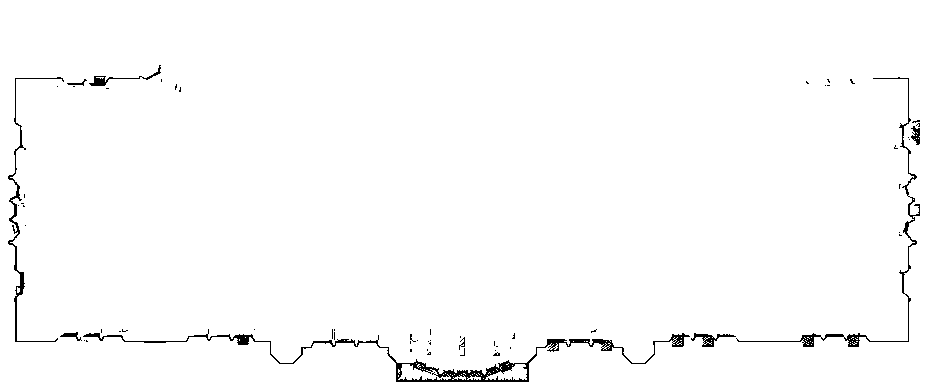
\includegraphics
        [width=0.4\textwidth]
	{figures/image_slice_0190.png}
	}
  }
  \subfloat[]{
    \label{fig_slicing:b} %% label for first subfigure
    \fbox{
    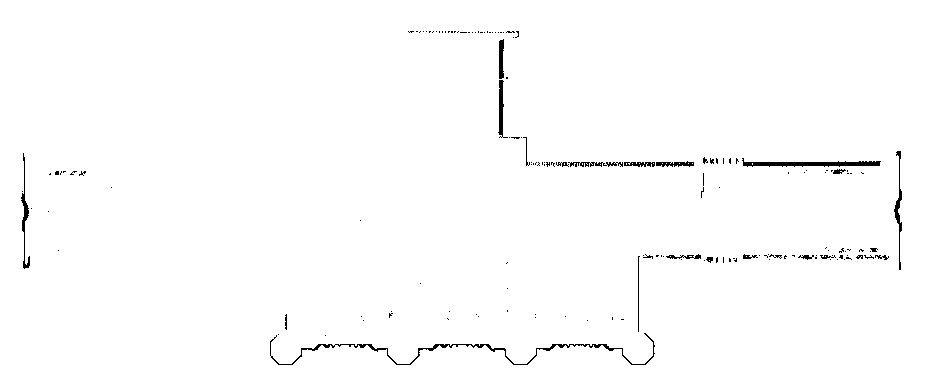
\includegraphics
        [width=0.4\textwidth]
	{figures/image_slice_0714.png}
	}
  }
  \vspace{.01in}
  \subfloat[]{
    \label{fig_slicing:c} %% label for first subfigure
    \fbox{
    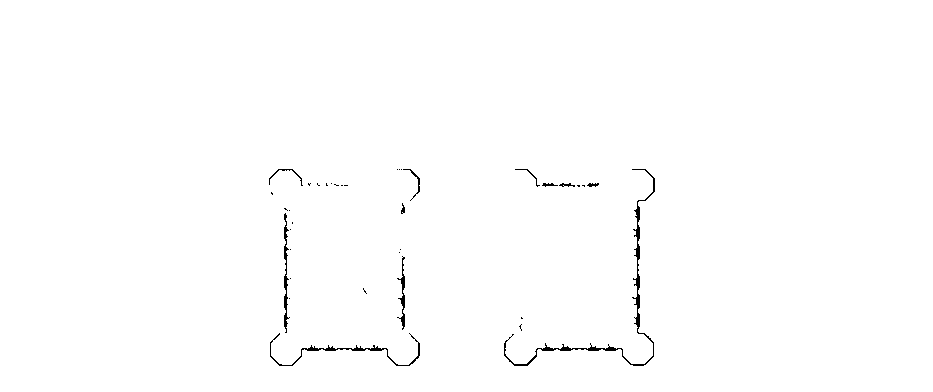
\includegraphics
        [width=0.4\textwidth]
	{figures/image_slice_0886.png}
	}
  }
  \subfloat[]{
    \label{fig_slicing:d} %% label for first subfigure
    \fbox{
    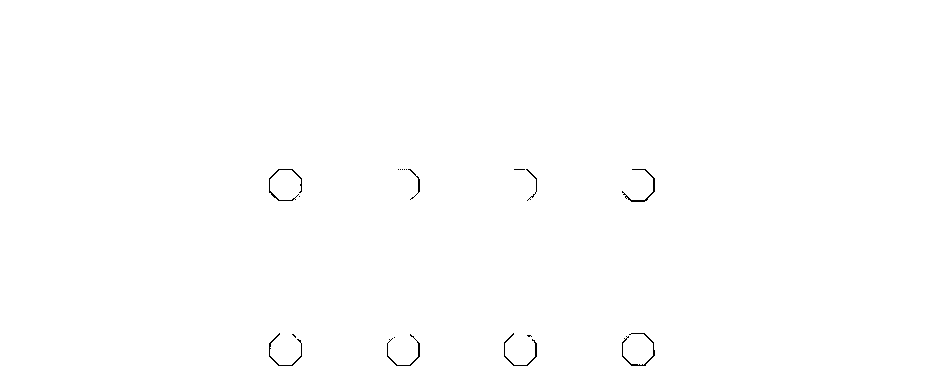
\includegraphics
        [width=0.4\textwidth]
	{figures/image_slice_0951.png}
	}
  }
  \caption{
The samples of 2D sliced images.
}
  \label{fig_slicing}
\end{figure}

Without loss of generality, the $y-$axis is used to represent the bottom-up
vertical direction.
We project the 3D data
$\boldsymbol{P}(x,y,z), H_{lo} \leq y < H_{hi}$, in the height range
$[H_{lo}, H_{hi})$ onto a 2D image slice.
The projection is normalized in the range $[0,W]$,
where $W$ is the image width:
\begin{equation}\label{eq_image_slicing}
[\,x^{2D},\; y^{2D}\,]^T = \omega\cdot[\,x^{3D}_i - X_{MIN},\; z^{3D}_i - Z_{MIN}\,]^T
\end{equation}
Note that $\omega = W/(X_{MAX} - X_{MIN})$, and that
the [$X_{MIN}$, $X_{MAX}$] and [$Z_{MIN}$, $Z_{MAX}$] pairs define the
3D bounding box, which can be obtained through user input and can be used
to clip away noise data. Fig. \ref{fig_slicing}(a)-(d) show some examples of the
2D slices, where noise and incomplete data are observed.

\subsubsection{Missing Data Recovering}
\label{sec_mdr}
The slices we extract above are often filled with holes due to occlusion
or other visibility issues.
Fortunately, most urban buildings have symmetry that we can exploit to
fill these holes.
Symmetry computation on 3D data \cite{Sym_PSGRF,Sym_ZPA,Sym_TW,Sym_MGP} is expensive,
so we conduct this computation on the 2D image slices.
Since the 3D data has been already rectified \cite{RDP_LSYGS} and projected onto 2D slices, hence only 2D translation
is needed to be considered for symmetry computation.
Let $P(x,y)$ be a point on the original image $I$ and $P'(x',y')$ be the reflected
point of $P$ with respect to a symmetry line $L$.
The symmetry computation equation for $L$ is as follows:
\begin{equation}
L = \underset{x,y}{\operatorname{arg\,min}}\sum{d_{x,y}(P', I)}
\end{equation}
where the $d_{x,y}(P',I)$ is the distance between the self-reflected point
$P'$ and its nearest data point in image $I$.
The reflected point $P'$ of the original point $P$ is computed with
respect to a line along either the $x-$ or $y-$ axis.
Therefore, the symmetry line $L$ is obtained as the line with minimum
summation error over the reflected data points.


%%%%%%%%%%%%%%%%%%%%%%%%%%%%%%%%
%%%%%%   3D Reconstruct  %%%%%%%
%%%%%%%%%%%%%%%%%%%%%%%%%%%%%%%%
\subsection{Lightweight 3D Reconstruction}
\label{sec_reconst}
Our 3D reconstruction algorithm is based on \emph{a priori} knowledge that
urban buildings can be created through a series of extrusion and taper
operations on the salient cross-sections contained in the keyslices.
It is therefore critical to identify those salient cross sections upon
which the extrusion and taper operations will apply.
This will be the key step for successful modeling.

\subsubsection{Extrusion Detection}
\label{sec_ksd}
The 2D image slices of an extruded region are similar to each other.
Thus, to detect an extrusion region one only needs to compute
the similarity between adjacent slices.
In other words, the sliced images are clustered into different groups based on the similarity among them.
There are two mainly research methods for similarity measurement of 2D images: area based method and feature based
methods. The area based methods are computational efficient but they usually can only be applied on
binary or gray-scale images. The feature based one is computational complex but more powerful and can be applied
to images obtained using different sensors, such as multi-modal image registration.
Because our goal is to develop lightweight efficient algorithm for model reconstruction, plus
the input for similarity measure is pure binary images, the area based method is adopted for our approach.

For 3D modeling of urban buildings, we are only interested in the boundary or silhouette of building.
Therefore, an image sweeping process is carried out for sliced images to obtain the boundary pixels
of each sliced layer. To measure the similarity of these boundary images, we adopted the Hausdorff
distance as the criterion for comparison.
\\
\\
\textbf{Hausdorff Distance}
\\
\\
Let $P_r(x_r, y_r)$ be a data point in a reference image and
let $P_i(x_i, y_i)$ be a data point in a new observed image $I$.
The Hausdorff distance of image $I$ to reference image $I_r$ is defined as:
\begin{equation} \label{eq.hd}
d_H(I, I_r) = \sum_{i=0}^Nd_{min}(P_i, I_r)
\end{equation}
where $d_{min}(P_i, I_r)$ is the minimum distance from data point $P_i$
in image $I$ to the reference image $I_r$.
Alternatively, we can also define the Hausdorff distance, $d_H(I_r, I)$,
from reference image $I_r$ to a new observed image $I$, using the equation \ref{eq.hd}.
These two distances are usually not equal to each other.
As a rule of thumb, one can choose
$d_{HD} = \text{MAX}\{d_H(I, I_r), d_H(I_r, I)\}$ as the Hausdorff distance.
To compute the keyslices, a threshold $\tau_{d}$ is used for the
Hausdorff distance $d_{HD}$.
If $d_{HD} < \tau_{d}$, the two images $I$ and $I_r$ are considered
similar to each other.
Otherwise, a keyslice image is found and $I_r$ is updated with $I$,
the new keyslice image.

The accuracy of the keyslices detected by using the Hausdorff distance
is mainly dependent on the threshold $\tau_d$.
Small $\tau_d$ leads to more accurate models and will require more time and
space to compute and store the result.
Therefore, there is a trade-off between model accuracy and time-space
efficiency.
This leads to an issue that some keyslices with salient feature may be missed in the web-based application where
the threshold $\tau_d$ is relative large in order to keep the time and space efficiency.
To conquer this problem, the curvature information is computed as a complementary
criteria for the keyslice detection.
\\
\\
\textbf{Curvatures Computation}
\\
\\
This idea is based on the observation that the keyslices are generally located at
the places where the curvature of the orthogonal direction changes as shown in Figure
\ref{HT_BPA_Curvature}\subref{HT_BPA_Curvature:a}. Therefore,
instead of computing the difference between two images directly, we can compute the
curvature in the orthogonal direction, and map those places where the curvature changes
back to the corresponding locations of slabs and mark them as keyslices.

\begin{figure}[htbp]
  \centering
  \subfloat[]{
    \label{HT_BPA_Curvature:a} %% label for first subfigure
    \fbox{
      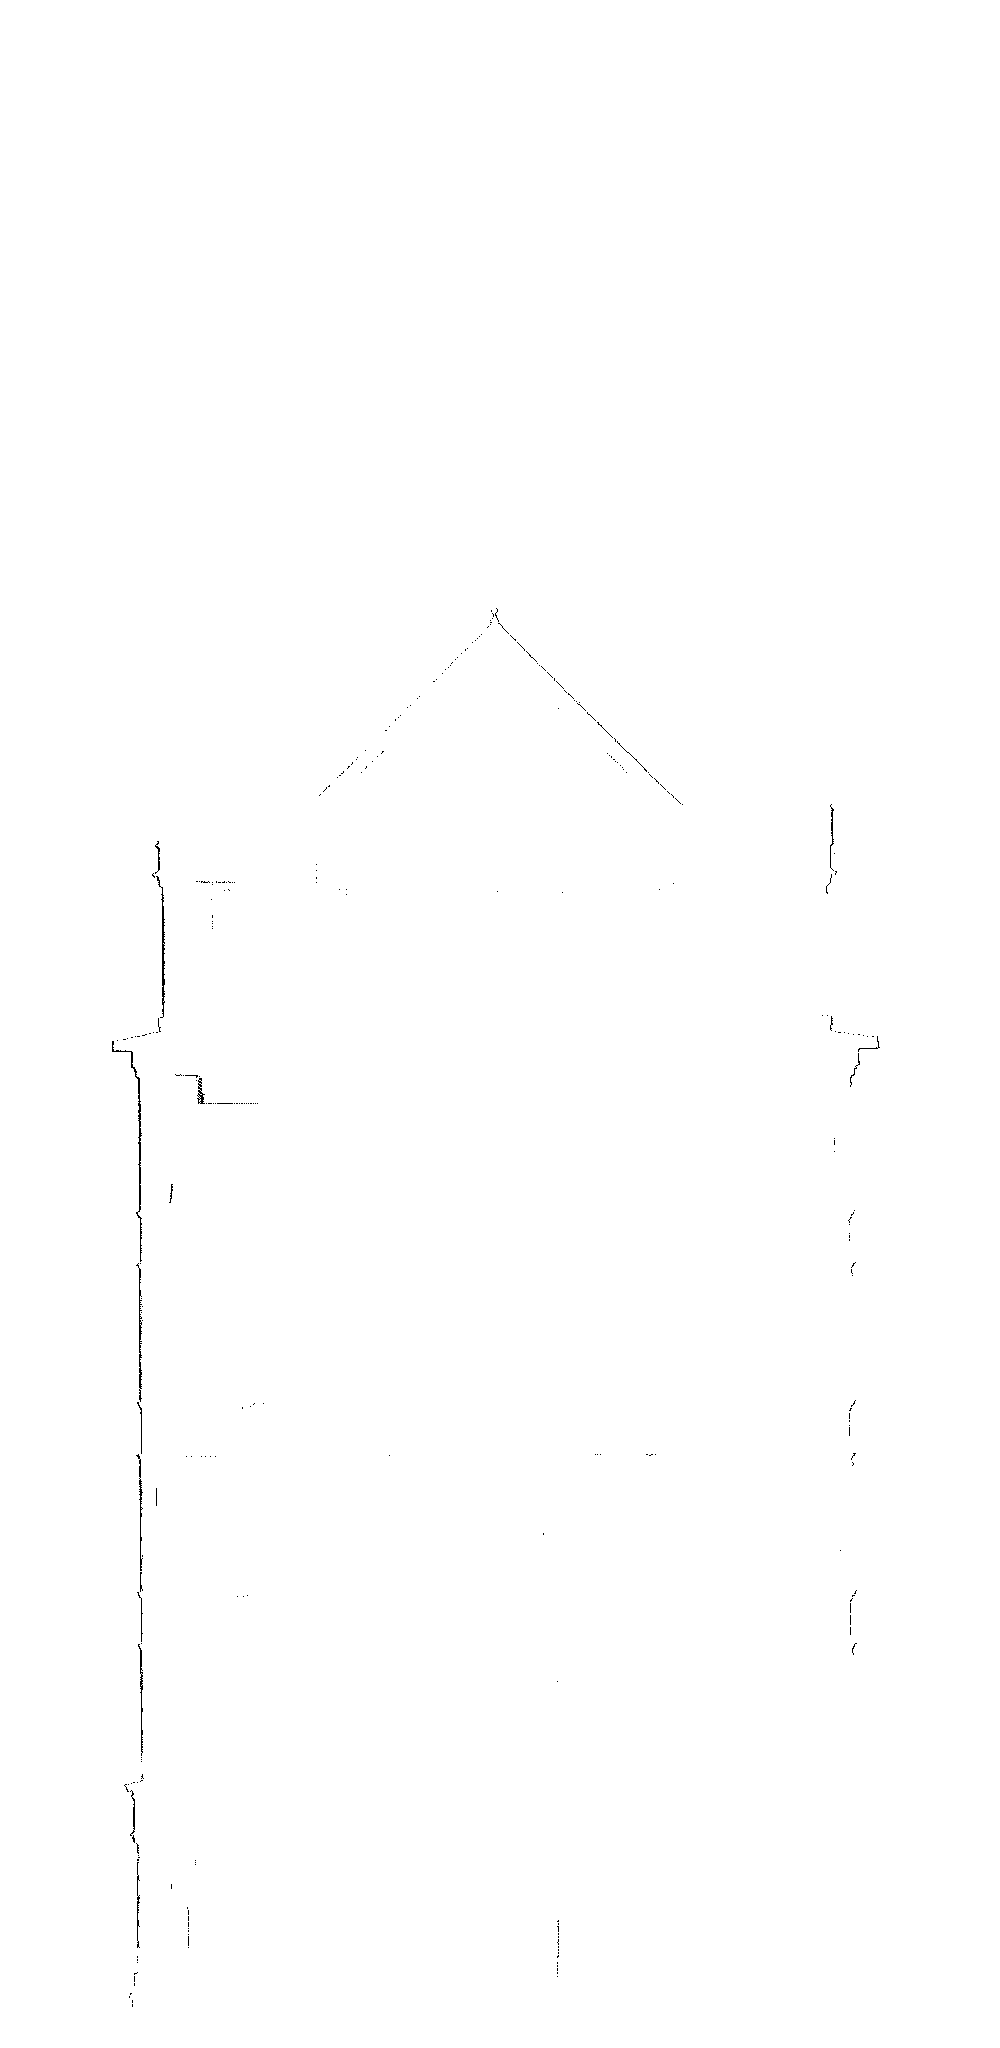
\includegraphics
	  [width=0.45\textwidth]
	  {figures/image_slice_1024_392_0820.png}
    }
  }
  \subfloat[]{
    \label{HT_BPA_Curvature:b} %% label for second subfigure
    \fbox{
      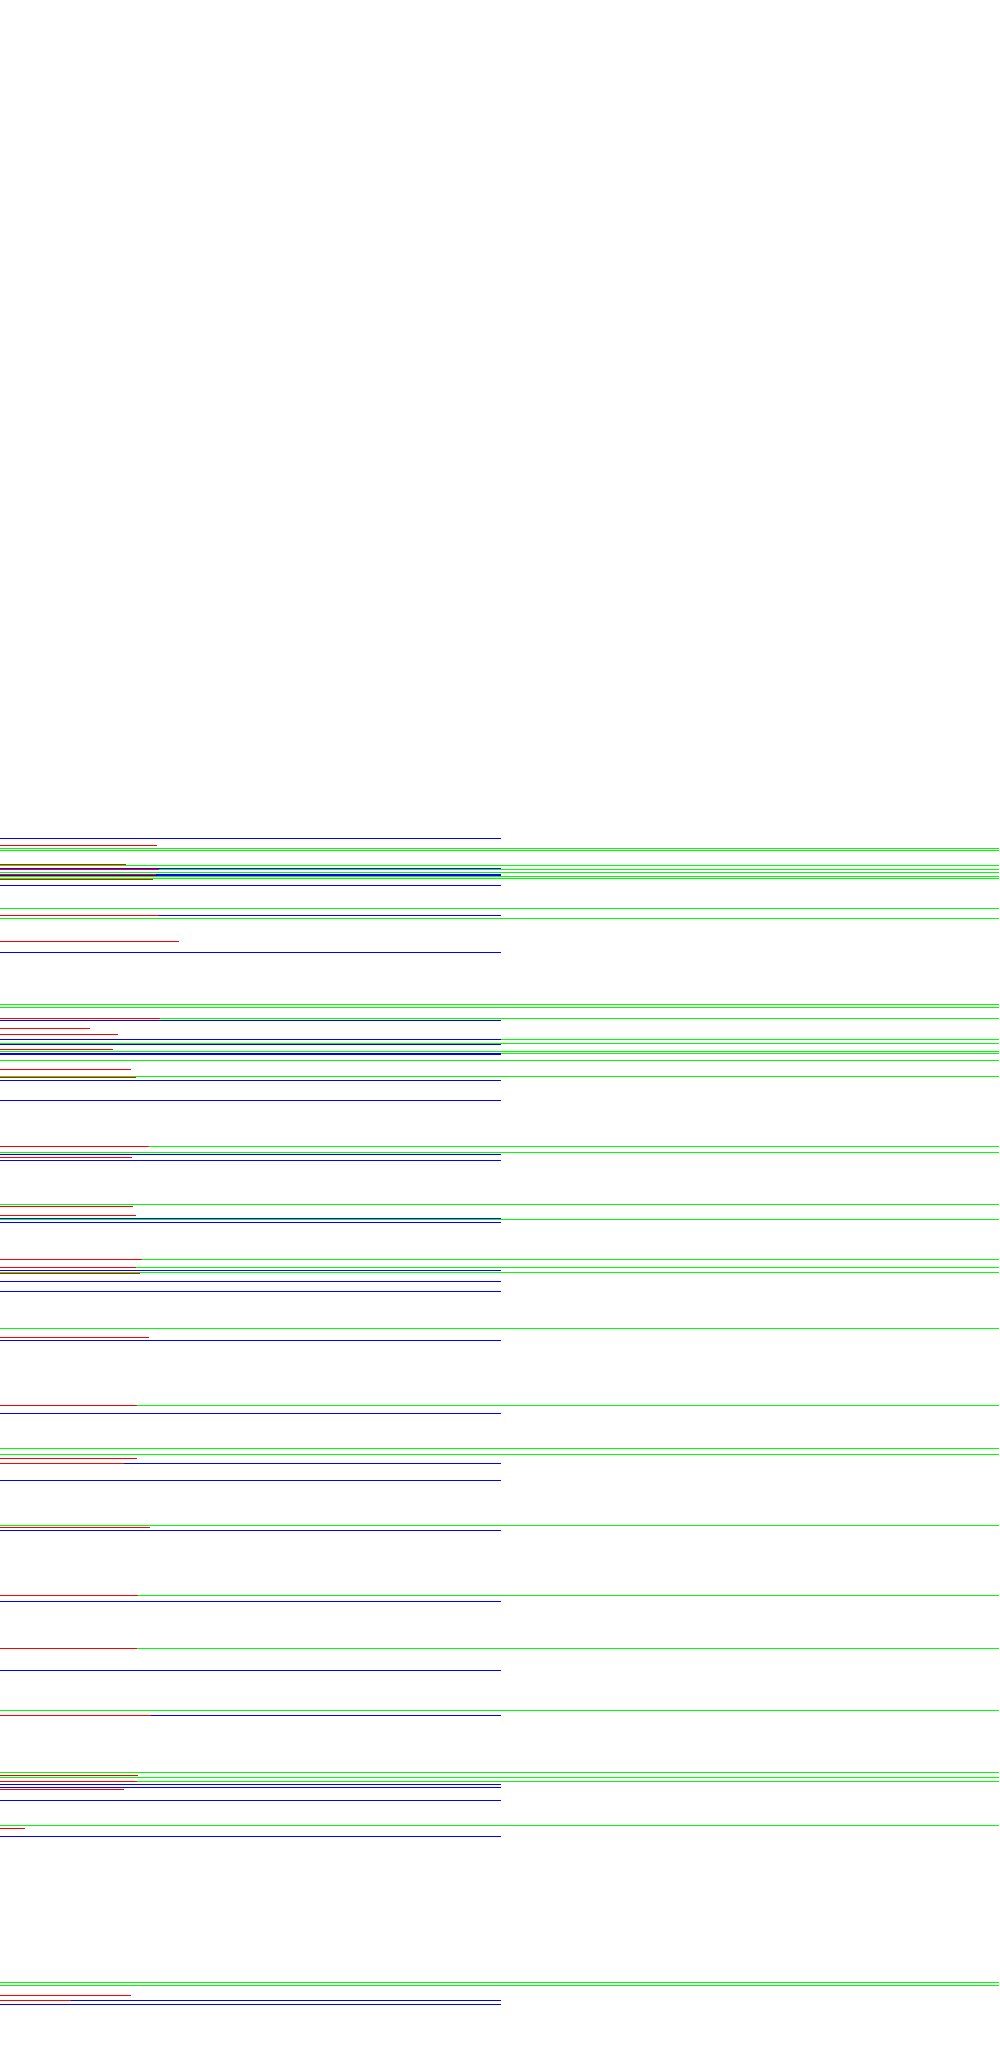
\includegraphics
	  [width=0.45\textwidth]
	  {figures/curvature_center_lines.png}
    }
  }
  \caption{ Curvature based key slice detection. (a) A slice image from the orthogonal direction.
(b) The average curvatures detected by a series of sliced image. }
  \label{HT_BPA_Curvature}
\end{figure}

To compute the curvature, we first apply the slices extraction algorithm described in Section
\ref{sec_image_slicing}
to obtain a series of 2D cross-sectional images in the orthogonal direction. After that, we applied
ball-pivot algorithm described in Section \ref{sec_BPA} to vectorize the boundary for each
sliced image. We located those curvatures that appear in most of the sliced images as the
places where keyslices are found as shown in Figure \ref{HT_BPA_Curvature}\subref{HT_BPA_Curvature:b}, where the red lines
indicate location of the center of the curvature, the blue and green lines indicate the
entering and exiting of the curvature structures. The combination of Hausdorff distance measurement
and curvature inference ensures that the salient structures of a building will be
preserved as well as the time and space efficiency for web-based applications.

\subsubsection{Boundary Vectorization}
After the key slices detection, $N_K$ key sliced images could be identified from the total $N_A$ sliced images.
Depend on the threshold $\tau_{d}$, $N_K$ is usually about 1 - 2 order smaller than $N_A$,
e.g., $N_K/N_A$ is 0.06 when $\tau_d$ = 4.0 for the example in Figure \ref{fig_IR_2_DXF}\subref{fig_IR_2_DXF:a}.
 Once we obtained these $N_K$ key sliced images, the next step is to vectorize these raster images for modeling.

As we mentioned earlier, because of missing data which produces gaps between structures, it
is generally hard to determine an appropriate radius, $r$, of the pivoting ball in advance.
To solve this problem, a coarse-to-fine, adaptive ball-pivot algorithm is proposed.
The basic idea is to start with a relative big $r$ ( ensure the gap will be covered by the ball of radius $r$) as
a coarse step for the initial BPA to guarantee that the ball will travel all boundary data before
turning back or reaching any existed boundary points. After this, a refinement process
is applied on the obtained points to get more accurate results with smaller $r$.
The refinement will stop when $r$ is reduced to be less or equal to the threshold $\tau_r$.
\\
\\
\textbf{Ball-Pivot Algorithm}
\label{sec_BPA}
\\
\\
Ball-pivot algorithm which was original proposed by Bernardini et al. in \cite{BPA_BMRS} is an
efficient technique for 3D range data surface reconstruction. Because of its simplicity and efficiency,
we apply this algorithm on 2D image for boundary vectorization. The basic idea of the BPA algorithm is
shown in Figure \ref{fig_BPA}(a): pivot a ball or a circle on the data point, mark those points (in red)
which are touched by the ball. Keep doing the pivoting process until the ball could not touch any new points.
Although the basic idea is straight-forward, the implementation of BPA is not a trivial work.
A bad implementation has a significant impact on the efficiency and effective of the algorithm.
\\
\\
\textbf{The Refinement of the BPA}
\\
\\
The output $\boldsymbol{\Phi}$, from the initial BPA, contains an ordered list of the boundary data
points $\boldsymbol{P}$ and their corresponding directions $\overrightarrow{\boldsymbol{R}}$ in which
the circle $C$ starts pivoting.
Because of the large radius $r$ in the initial BPA, $\boldsymbol{\Phi}$ is just a coarse representation
of the boundary and needs to be refined.

\begin{figure}[htbp]
  \centering
  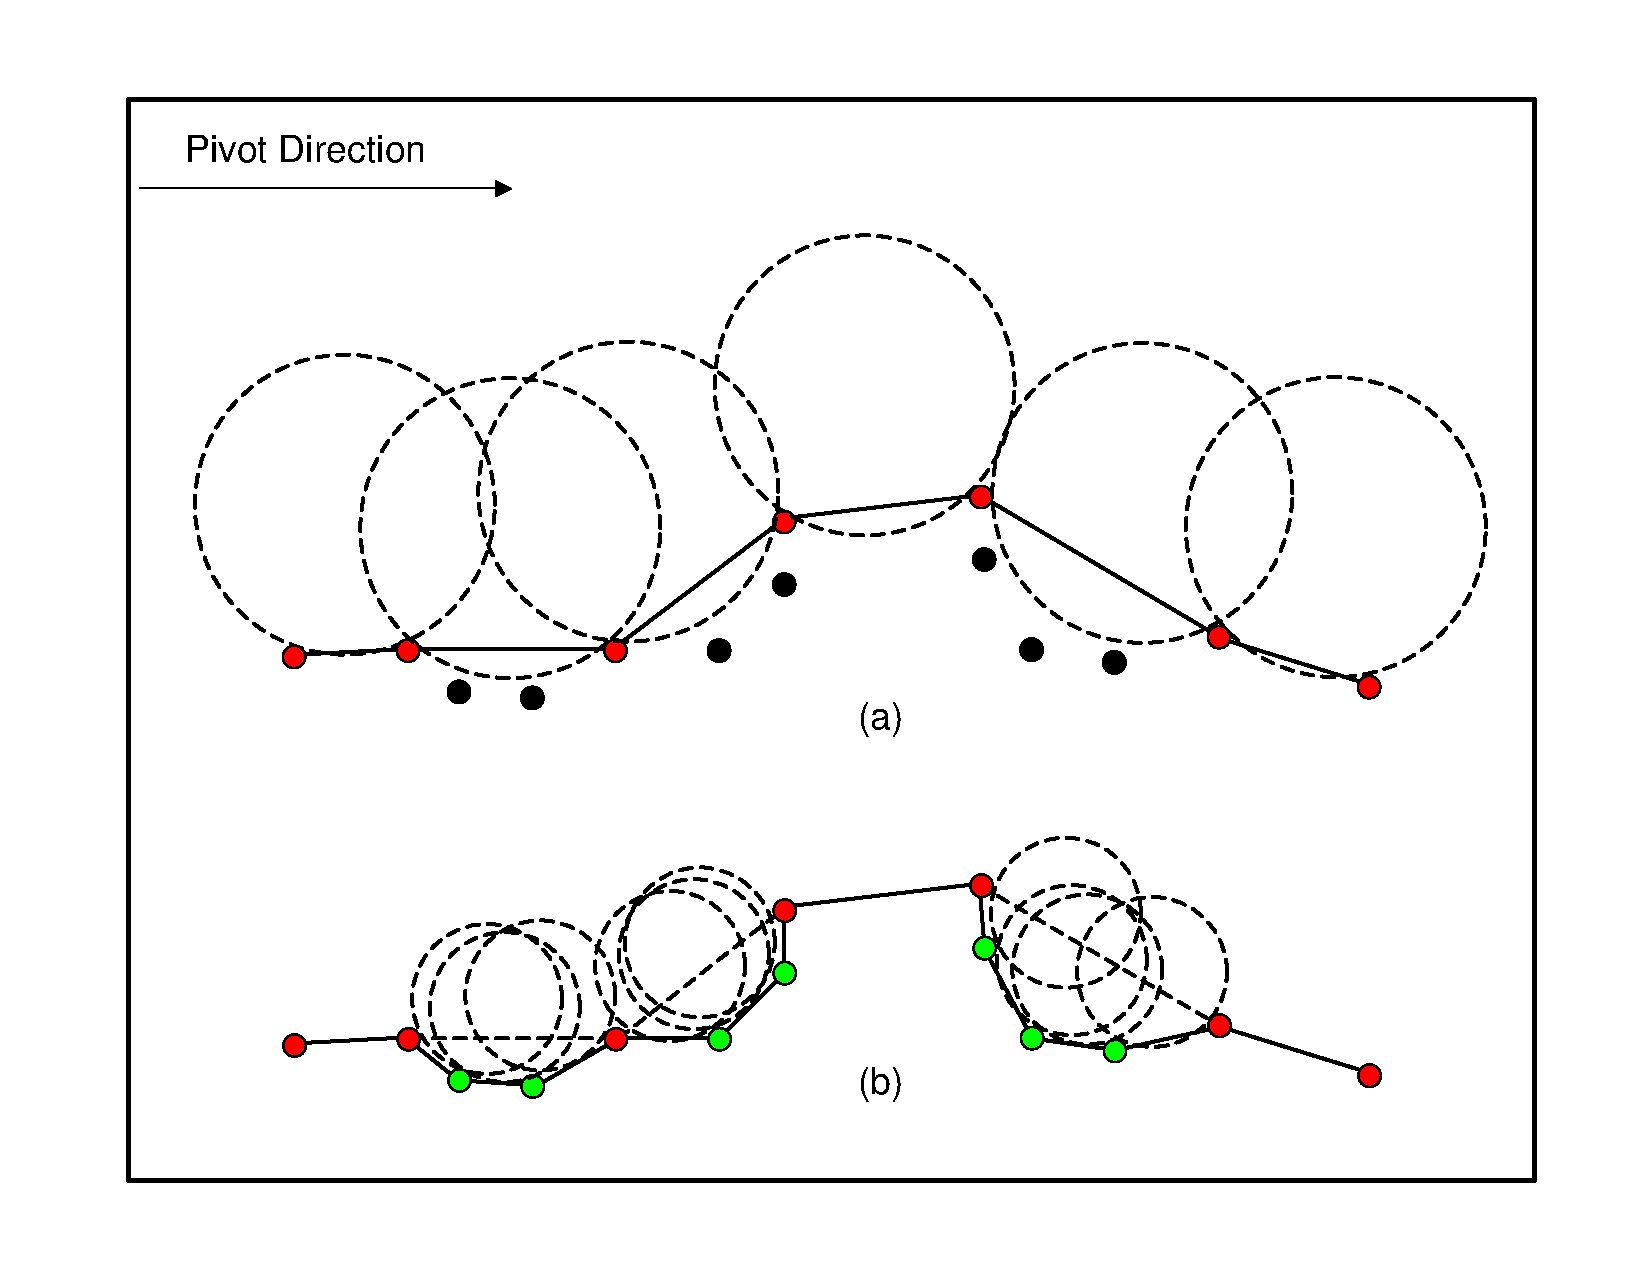
\includegraphics
      [width=0.8\textwidth]
      {figures/BPA.pdf}
      \caption{Ball pivot algorithm: (a) Initial pivoting with circle of radius 2$r$
	(b) Refinement process with circle of radius $r$.}
      \label{fig_BPA}
\end{figure}

The refinement algorithm is based on an iterative process with respect to the circle
radius $r$ as shown in Figure \ref{fig_BPA}(b). For each iteration, the radius of
the circle is reduced, e.g., $r' = r/2$. Then the length of the line segment formed by adjacent points
is checked, $\ell = \overline{P_0P_1}$, in $\boldsymbol{\Phi}$.
If this line is shorter than the new radius $r'$, it is ignored at this iteration. This is
because we can always leave short lines refinement to next rounds if needed.
If refinement is needed on $\ell$, the BPA algorithm with updated radius $r'$
is applied with parameters $\boldsymbol{S} = (P_0, \overrightarrow{\boldsymbol{R_0}})$.
That is, it takes the first point $P_0$ and its direction $\overrightarrow{\boldsymbol{R_0}}$
as input parameters. The BPA starts with the new circle $C'$ of radius $r'$, and
stops when either it reaches the end point $P_1$, or it turns back at a place where
the refinement ball size $r'$ is smaller than the gap between two data points.
If it reaches $P_1$, which means this pivoting process is valid, a new list
of ordered boundary points, $\boldsymbol{\Phi'}$, would be inserted into
$\boldsymbol{\Phi}$ between $(P_0, \overrightarrow{\boldsymbol{R_0}})$ and
$(P_1, \overrightarrow{\boldsymbol{R_1}})$.
On the other hand, If the circle $C'$ can not reach $P_1$, the new obtained
$\boldsymbol{\Phi'}$ would be discarded.
When the pivoting reaches the last point in the ordered list $\boldsymbol{\Phi}$,
this iteration with radius $r'$ ends.
The refinement algorithm repeats the iteration process until the new radius $r'$ is
smaller than the threshold $\tau_r = \omega * \tau_d$, where $\tau_d$ is the threshold for Hausdorff distance
and $\omega$ is a scale factor for the threshold $\tau_r$ with respect to $\tau_d$.
\\
\\
\textbf{The Integration of BPA and HT}
\\
\\
Although the adaptive BPA is a very efficient and straight-forward approach to vectorize
the boundary or silhouette of raster images, it is prone to the noise. This is illustrated
in Figure \ref{HT_BPA_figure}\subref{HT_BPA_figure:a}. As we can see, the upper part of the vectorized image
contains some bogus detailed structures which actually belong to the same line structure. In the
case where the outlier is not close enough to the real data, the result will be significantly
degraded. Based on the observation that most of the boundaries of the man-made building
are of line structures, we can improve the adaptive BPA results by incorporating the line
information.

\begin{figure}[htbp]
  \centering
  \subfloat[]{
    \label{HT_BPA_figure:a} %% label for first subfigure
    \fbox{
      \includegraphics
          %[angle=90, scale=0.25]
          [width=0.75\textwidth]
	  {figures/bbb_image_slice_1024_392_0533_refine_with_rad_1_and_merged.png}
    }
  }
  \vspace{.2in}
  \subfloat[]{
    \label{HT_BPA_figure:b} %% label for second subfigure
    \fbox{
      \includegraphics
          %[angle=90, scale=0.25]
          [width=0.75\textwidth]
	  {figures/bbb_image_slice_1024_392_0533_combine_HT_BPA_rad_32.png}
    }
  }
  \caption{ (a) a sliced image vectorization with adaptive BPA
(b) the combination of hough transform and BPA on the sliced image. }
  \label{HT_BPA_figure}
\end{figure}

To combine the adaptive BPA with HT, we first apply our adaptive HT algorithm on the raster
image to obtain all lines $\boldsymbol{L}$ and sort them from the longest to the shortest one.
Generally speaking, the longer lines give more confidence on the line structure of the building.
For integration, we first apply dilation operation on $I$ using 8-connected kernel
to get the dilation image, $I_d$. The next step is to measure how well the lines in
$\boldsymbol{L}$ match the data in $I_d$, which determines whether a line in $\boldsymbol{L}$
should be used as a substitution or not.

If a line segment $L$ is found to be a good candidate, the next step is to find the corresponding part of the
BPA points in $\boldsymbol{\Phi}$ for substitution. To do this, we first compute the closest two points
$P_i$ and $P_j$ in $\boldsymbol{\Phi}$ to the two end points of $L$.
Generally speaking, the points in $\boldsymbol{\Phi}$ represent a polygon and therefore form a circle layout, i.e.,
$\boldsymbol{P} = \{ P_0,P_1,\ldots ,P_{n-1}, P_0 \}$. Assume $i < j$, there are two possible choices to replace
the series of the points, which are
$\boldsymbol{P_1} = \{ P_i,P_{i+1},\ldots,P_{j-1}, P_j \}$, and
$\boldsymbol{P_2} = \{ P_j,P_{j+1},\ldots,P_{i-1}, P_i \}$.
To determine which one is correct, one can compare the distance, $D$, from the line $L$ to both
set of the points $\boldsymbol{P_1}$ and $\boldsymbol{P_2}$. The point set with smaller $D$ is
about to be substituted by the line $L$.
\begin{equation*}
D = \underset{\boldsymbol{P_1},\boldsymbol{P_2}}{\operatorname{arg\,min}}\sum{\lVert P_i - L \rVert}
\qquad P_i \in \boldsymbol{P_1} \ \text{or} \ P_i \in \boldsymbol{P_2}
\end{equation*}
where $\lVert P_i - L \rVert$ is the Euclidean distance from a point $P_i$ to the line $L$.

%%%%%%%%%%%%%%%%%%%%%%%%%%%%%%%%%%%%%%%
%%%% Let's describe this in thesis %%%%
%%%%%%%%%%%%%%%%%%%%%%%%%%%%%%%%%%%%%%%
%\subsubsection{The Implementation of Adaptive BPA}

%Describe the global threshold and settings?

\subsubsection{Tapered Structure Detection}
\label{sec_tsd}
After the keyslices are detected and vectorized, the silhouettes of
$N_K = \{I_{i}, i = 0, ..., K \}$ keyslices
can be used to represent the whole building based on the extrusion operation.
That is, the space between each pair of keyslices, say $I_{i}$ and $I_{j}$,
can be interpolated by the lower keyslice, e.g., $I_{i}$ in this case.
This is valid due to the similarity between the intermediate images and the
keyslice $I_{i}$.
By modeling a building using this series of keyslices $N_K$, we can largely
reduce the space needed to store urban buildings.
This helps make possible 3D web-based applications such as 3D city navigation.

In addition to the extrusion operation, we can further improve the model
and reduce the model size by observing that part of the keyslice images
belong to the same tapered structure.
This is demonstrated in Figure \ref{fig_DXF_top}.
Figure \ref{fig_DXF_top}\subref{fig_DXF_top:a} shows the roof structure
of the reconstructed model based on a keyslice image extrusion operation with
almost half of the keyslice images dedicated to the roof structure.
After applying the tapered structure inference,
Figure \ref{fig_DXF_top}\subref{fig_DXF_top:b}
shows the improvement of the modeling.
As we can see, the roof in Figure \ref{fig_DXF_top}\subref{fig_DXF_top:b}
is much smoother than that in Figure \ref{fig_DXF_top}\subref{fig_DXF_top:a}.
In addition, the keyslices needed to represent the building, and its
associated storage, are reduced almost in half.

The difficulty of inferring tapered structure lays on the complication of
the building structure itself.
Let's assume that the height range for roof structure is
$H_R = [H_{lo}, H_{hi}]$.
If this is the only existing structure between $H_R$, it is simple and
straight-forward to detect and infer this part.
%Namely, we only need to find the corresponding feature points between the bottom
%the top feature points.
However, for some complicated structures, such as a mixed layout
of tapered and extruded structures, some special treatment is needed to obtain
the desired results.
Our approach is based on the divide and conquer strategy: the whole
structure $\boldsymbol{U}$ is segmented into independent sub-structures,
$U_0, U_1, \ldots, U_N$. For any sub-structure $U_i$,
it contains only a unique structure, either a tapered or an extruded one. Once
each unit $U_i$ is inferred, the whole structure can be modeled by an union operation
of these sub-structures, i.e., $\boldsymbol{U} = \bigcup{U_i\{ i = 1,\ldots,N\}}$.
Before segmentation, the potential height ranges $H_R$ containing the tapered structures should be computed.
This can be done by checking the frequency of the keyslice images.
The structure containing tapered sub-structures will show a high and even
distributed keyslice images. This is a very useful clue for $H_R$ detection.

%%% Figure of the tapered template.
\begin{figure}[htbp]
  \centering
  \subfloat[]{
    \label{fig_DXF_top:a} %% label for first subfigure
    \includegraphics
        [width=0.8\textwidth]
%	{figures/BPA_250_top_crop.png}
	{figures/extrude_1.png}
  }
  \vspace{.5in}
  \subfloat[]{
    \label{fig_DXF_top:b} %% label for first subfigure
    \includegraphics
        [width=0.8\textwidth]
%	{figures/BPA_250_top1_crop.png}
	{figures/extrude_2.png}
  }
  \caption{  The top view of the 3D building. (a) without tapered structure. (b) with tapered structure }
  \label{fig_DXF_top}
\end{figure}
%%% End of Figure

Once the potential height ranges $H_R$ is obtained,
the next step is to segment the whole structure $\boldsymbol{U}$ between $H_R$ into
sub-structures, $U_i, \; i = 0,\ldots,N$. This is again done by similarity measurement of sliced images
from orthogonal directions. As before, the 3D data points following inside the range of $H_R$
are projected along both left-right ($X$ axis) and face-inside ($Z$ axis) directions.
Then the keyslice detection is carried out based on Hausdorff distance similarity measurement for
both directions. These keyslices will segment the structure in $H_R$ into sub units of $U_0, U_1, \ldots, U_N$.

For each sub unit $U_i$, we have to know whether it represents an extruded or a tapered
structure. The method is to check in the keyslice image $I_k$ of $U_i$ whether there exists
a pattern where two lines intersect with some appropriate angle.
% as shown in Figure \ref{TSD_fig_tapered_template}.
If such a pattern exists in $I_k$, the
unit $U_i$ is marked as a tapered sub-structure. Otherwise, $U_i$ is marked as
an extruded sub-structure. If $U_i$ is an extruded unit, its silhouette from the
$y-$ axis is vectorized and is ready for the union operation to obtain $\boldsymbol{U}$.
On the other hand, if $U_i$ is a tapered unit, the bottom and top position have to be computed
so that it can be reconstructed. To do this, all line segments $\boldsymbol{L}$ in $U_i$
are computed using the Hough Transform and the
%described in Algorithm \ref{alg.AHT}.
intersection point $P_0$ of $\boldsymbol{L}$ indicates
the top position of the tapered unit. The other end points $P_i$ of $\boldsymbol{L}$ are also computed
to infer the bottom shape and position.


%%%%%%%%%%%%%%%%%%%%%%%%%%%%%%%%
%%%%%%   Experimental Results%%%
%%%%%%%%%%%%%%%%%%%%%%%%%%%%%%%%
\subsection{Preliminary Results}
\label{sec_IR_OUT}

The results of the extrusion and tapered structures computation,
together with raster image vectorization, are stored in the 2D
image coordinate system. To generate the final 3D model, these
data need to be transformed
back into the 3D world coordinate system.

\subsubsection{Model Generation}

Let $P(x,y)$ be a point in the 2D image coordinate system, and let
$P'(x,y,z)$ be the 3D world coordinate of $P$, where $y$ is the depth coordinate.
For all points in the same boundary layer or silhouette,
the points lay in the same plane and hence have the same value of $y$.
The equation for transforming $P$ back to $P'$ is a reverse transformation of $\boldsymbol{T_0}$
in the equation \ref{eq_image_slicing}:
\begin{equation}\label{eq_ir2dxf}
[\,x^{3D},\; y^{3D},\; z^{3D}\,]^T = [\,\eta\cdot x^{2D} + X_{MIN},\; \zeta + Y_{MIN},\; \eta\cdot z^{2D} + Z_{MIN}\,]^T
\end{equation}
where $\eta=1/\omega$ and $\zeta=\kappa\cdot\delta$. Here, $\kappa$ is the index of the 2D slice and $\delta$
is the height of a slab described in the Section \ref{sec_image_slicing}.
Figure \ref{fig_IR_2_DXF}\subref{fig_IR_2_DXF:c} shows an exterior 3D model
generated by the above transformation.

\subsubsection{Error Measurement}
To measure the error between a reconstructed 3D model and its original point cloud,
we first mapped the generated model back to the 3D point cloud coordinate system.
The error is measured as the distance from the sampled 3D cloud data to their closest model planes, which
is computed using the following formula:
\begin{equation}\label{eq_em}
E = \frac{1}{|X|}\sum_{x\in{X}}{d^2(x, M)}
\end{equation}
where $X$ is the set of 3D point cloud data. The distance
$d(x, M) = \text{min}_{p \in M}\lVert x - p \lVert$ is the minimum Euclidean distance from
a 3D point $x$ to its closest face $p$ of $M$.

\begin{table}[hbtp]
\centering
  \begin{tabular}[t]{||c||c|c|c||}
    \hline
    $\tau_{d} $(pixel) & Error (mm)& \# of faces & Size (KB) \\
    \hline \hline
    64 & 0.658 & 1471 & 15\\   %   64 & 9.63 & 1471 & 15\\
    \hline		      %   \hline		
    32 & 0.294 & 3284 & 32\\   %   32 & 4.30 & 3284 & 32\\
    \hline		      %   \hline		
    16 & 0.141 & 8574 & 86\\   %   16 & 2.06 & 8574 & 86\\
    \hline		      %   \hline		
    8 & 0.131 & 13955 & 137\\  %   8 & 1.91 & 13955 & 137\\
    \hline		      %   \hline		
    4 & 0.094 & 27214 & 261\\  %   4 & 1.38 & 27214 & 261\\
    \hline		      %   \hline		
    2 & 0.088 & 31331 & 335\\  %   2 & 1.28 & 31331 & 335\\
    \hline		      %   \hline		
    1 & 0.083 & 32187 & 337\\  %   1 & 1.21 & 32187 & 337\\
    \hline
  \end{tabular}
\caption{
The error measurement with respected to Hausdorff distance threshold $\tau_d$.
The BPA radius threshold $\tau_r = 4$. }
\label{tbl_em}
\end{table}

The accuracy of the final model mainly depends on the threshold of Hausdorff distance $\tau_d$ as
well as the threshold of BPA refinement radius $\tau_r$. $\tau_d$ determines the accuracy of the key slices detection
and $\tau_r$ determines the accuracy of the boundary vectorization.
Table \ref{tbl_em} lists the relationship among the $\tau_d$, errors, number of faces and model size.
The unit for $\tau_d$ is in pixels and for errors is in millimeters.
Table \ref{tbl_em} lists the relationship among the $\tau_d$, errors, number of faces and model size.
The size for original 3D building point cloud is more than 700 MB. From the table, one can see that even
for the most accurate model, the size is dramatically reduced compared with the original 3D point cloud data,
which is desired for web-based applications.

To visualize the error between real 3D data and inferred model, we generated the deviation
mapping images which are depicted in Figure \ref{fig_EM}. Basically, for each face $p$
of $M$, a corresponding texture image is computed. The intensity for each pixel of this image
is determined by the distance error of corresponding 3D data computed by Equation \ref{eq_em}.

%%% Figure of the tapered template.
\begin{figure} [hbtp]
  \centering
  \subfloat[]{
    \label{fig_EM:a} %% label for first subfigure
    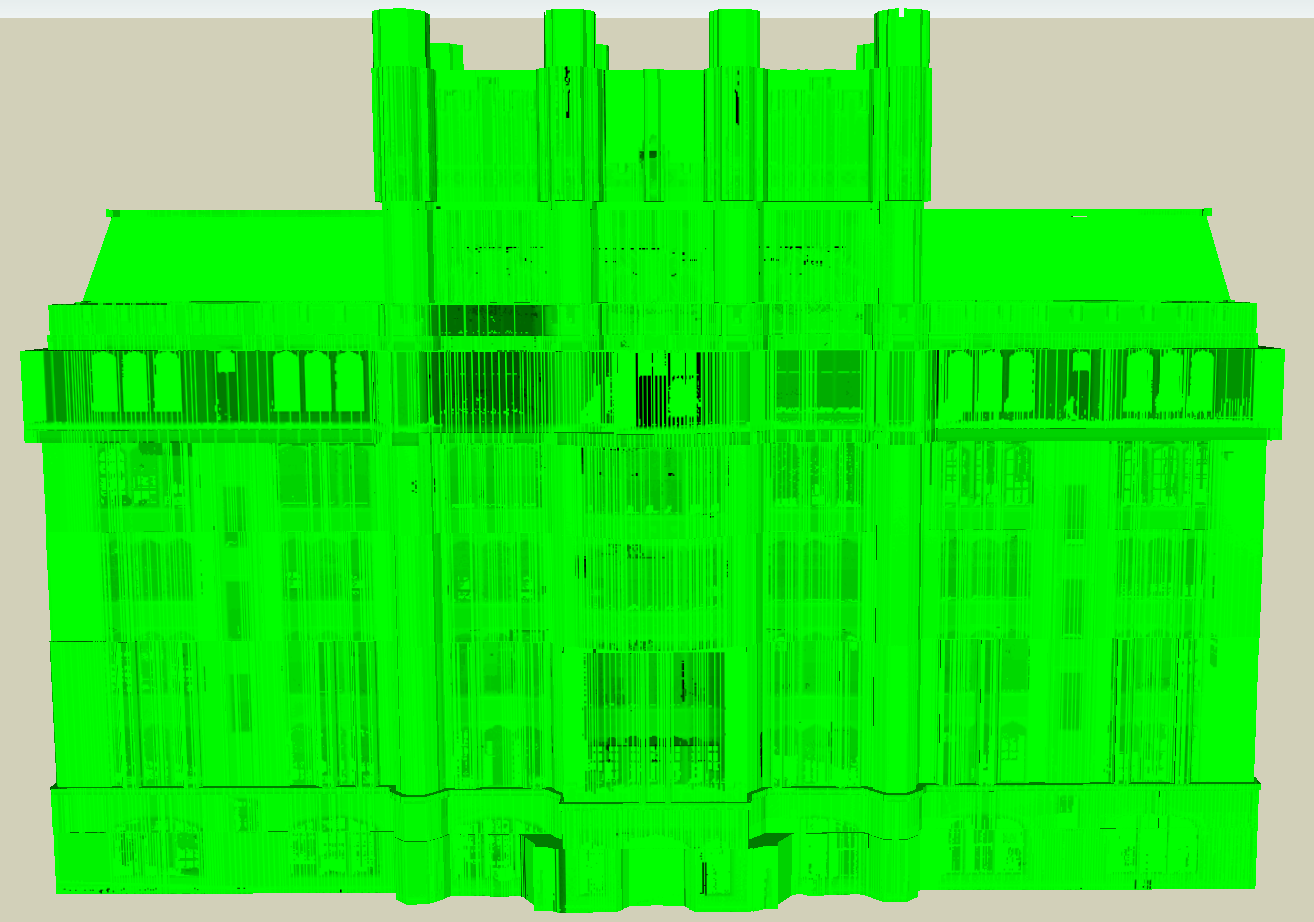
\includegraphics
        [width=0.8\textwidth]
	{figures/IR_skp_error_face_1000_32_4_paper.png}
  }
  \vspace{.5in}
  \subfloat[]{
    \label{fig_EM:b} %% label for first subfigure
    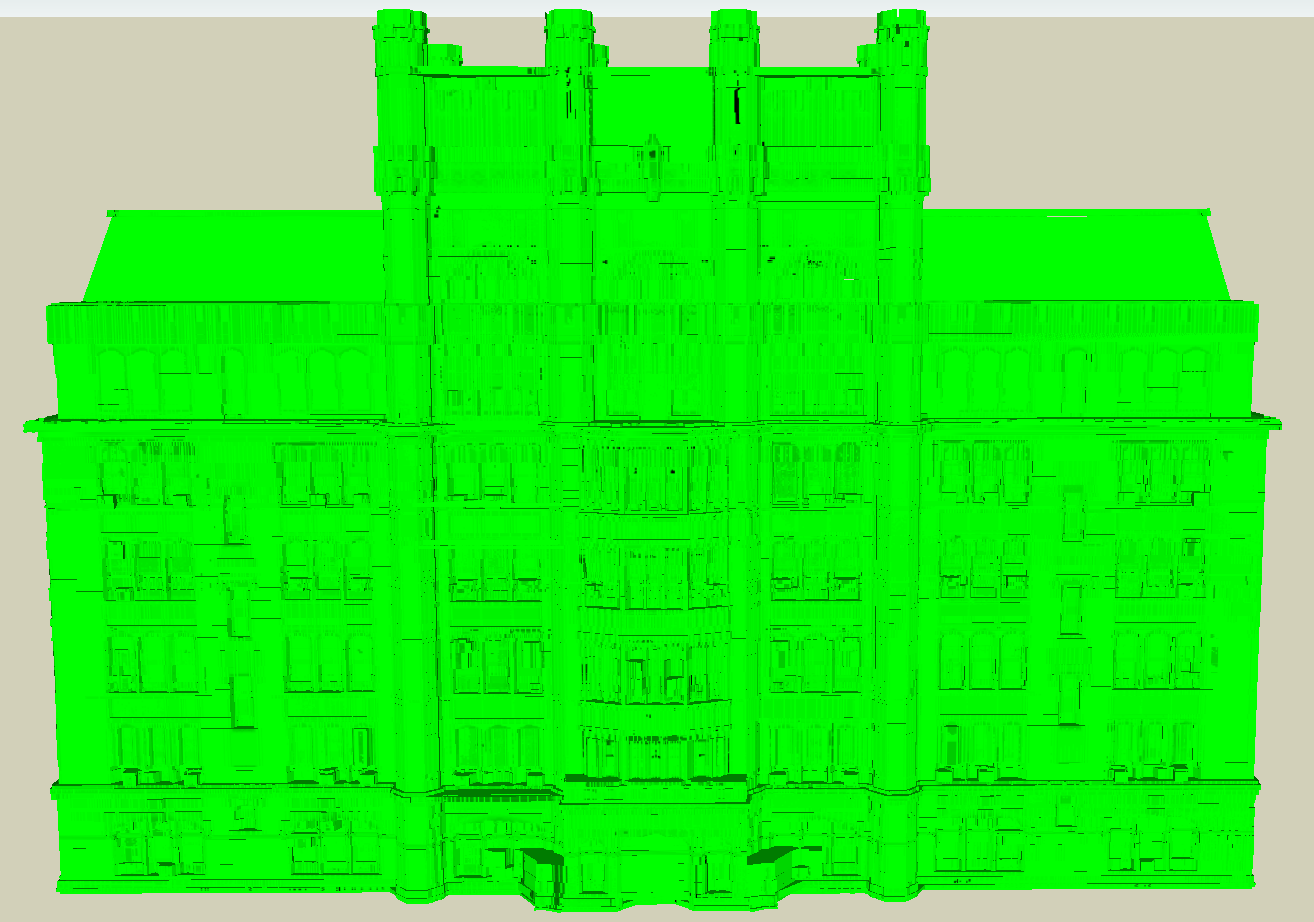
\includegraphics
        [width=0.8\textwidth]
	{figures/IR_skp_error_face_1000_4_1_paper.png}
  }
  \caption{  The deviation mapping of the 3D point cloud. (a) the model built with parameter of
$\tau_r$ = 4 and $\tau_d$ = 32. (b) the model built with parameter of $\tau_r$ = 1 and $\tau_d$ = 4. }
  \label{fig_EM}
\end{figure}
%%% End of Figure



\ifthenelse{\equal{\twocol}{true}}{
%\newpage % TWO COLUMN VERSION
}{
\newpage % TWO COLUMN VERSION
}
\section{Practical Aspects and Timeline}

In the processing of implementing the algorithm to obtain the preliminary results, we gained in-depth
knowledge of the 3D tools and related programming languages. The whole project consists of over 20,000
lines of C++ code and over 2,000 lines of Ruby code of Google SketchUp plug-ins for model visualization.
Based on the work has been done and this code base, we believe that the remaining research will
progress fast and the dissertation defense will be in September 2009.

The remaining research problems and the estimated timeline are listed in the following:
\begin{enumerate}

\item Investigate modeling of the tapering to a point geometry structure

We have successfully inferred the geometry structure of tapering to a line. As a further step, we will study
how to infer the geometry structure of tapering to a point which appears frequently in Gothic architecture,
like churches.
Our plan is to first segment out the region dedicated to this special structure.
This segmentation task can be done based on the connected components in the sliced 2D images.
Unlike the tapering to a line, we are not able to infer this structure by inferring extruded
structure from the orthogonal directions.
However, a nice characteristic of this structure is that
the sliced image will converge to a point, which is good clue for inference.
Without loss of generality, we assume that the sliced images of this special structure
can be vectorized by a closed polygon.
Let $S_i$, $S_j$ be two consecutive sliced images and $S_i$
has a smaller boundary than $S_j$. Based on this special structure, $S_i$ will be growing up
to cover $S_j$ by iterative dilation operations. By doing this, we can quickly locate the
bottom and top (a small region representing a point) slices of this special geometry
structure and therefore reconstruct this sub-model using these two slices.
The difference between this structure and the structure of tapering to a line is whether
$S_i$ and $S_j$ have any overlapping or common parts, which is easy to check.

The time needed to do this is about 2 weeks.
One and a half weeks will be dedicated to infer the underline structure.
The remaining time is used to create the sub-model.

\item Investigate modeling of the ``follow-me'' geometry structure

This useful feature is included in Google SketchUp, which inspires the paradigm used here.
``follow-me'' is a more complicated geometry structure which
exists when the underline geometry structure can be reconstructed by
moving a basic geometry unit along a curve trajectory.
We will carry out a tracking computation to obtain the curve trajectory.
To do this, we will first capture the base geometry unit from a projected 2D reference slice image $S_i$.
This base geometry is a very important initial stage because it is used as a template $A$
for the further tracking process.
Alternatively, to make this more precise or reliable, we could also get the base geometry part
of a reference image from user input.
Once the template $A$ is defined, we can start the tracking from the reference image along
two oppose directions, that is $i, i+1, \ldots$ and $i, i-1, \ldots$.
Because of the dense projection, the template matching based tracking process only needs to search
in a small local region.
This tracking process ends when no pattern is found in the new sliced images, which means the
boundary of this special structure is reached.

The estimated time needed to do is about 3 weeks.
Two weeks will be dedicated to the tracking of the base geometry
and the remaining time is used to compute the final model from the tracking results.

\item Performance evaluation with other techniques

We will conduct more advanced performance evaluation on the proposed approach, especially the
comparison on state-of-the-art techniques.
First of all, we will carry out the comparison on the high resolution models
generated with our proposed method and those generated by using ball-pivot algorithm.
The BPA is a very efficient algorithm and can generate precise models from range data with
a small ball radius.
To do the comparison, the number of faces or triangles in these high resolution models
from both methods will be approximately the same level.
The metric for comparison will include both objective and subjective criteria. The objective
comparison will measure the errors between the models and the raw range data.
And a subjective measurement will rely on sharpness of the models for the visualization.
On the other hand, we will also carry out the comparison on the low resolution models
generated by our methods and others, such as qslim approach.
The same comparison metrics used for high resolution models will be used here.

The estimated time for this is 2 weeks.
It takes about a week to download and get familiar with other tools, such as qslim. And then one more
week is needed to conduct the comparisons.

\item Carry out experiments on more complicated datasets

Currently we have only applied the proposed approach on one set of range data, which is a
exterior scanning of the buildings.
In order to test the effectivity and reliability the proposed algorithm,
we will carry out the experiments on more complicated point cloud datasets, such as
interior scanning of a large hall, where more sophisticated structures exist.
Roughly we will try the proposed approach on about half dozen of large-scale datasets to
validate our techniques.

The estimated time for this work is about 3 weeks.
The dataset may not be the same size but on average two datasets will be processed in each week.

\end{enumerate}


%%%%%%%%%%%%%%%%%%%%%%%%%%%%%%%%
%%%%%%   Bibliography %%%%%%%%%%
%%%%%%%%%%%%%%%%%%%%%%%%%%%%%%%%
\newpage
\bibliography{proposal}
\bibliographystyle{unsrt}

\newpage


%%%%%%%%%%%%%%%%%%%%%%%%%%%%%%%%
\end{document}
